\documentclass[9pt]{article}

\usepackage[utf8]{inputenc}
\usepackage[T1]{fontenc}
\usepackage{hyperref}
\usepackage{url}
\usepackage{booktabs}
\usepackage{amsfonts}
\usepackage{amsmath}
\usepackage{graphicx}
\usepackage{subcaption}
\usepackage{xcolor}
\usepackage{array}
\usepackage[margin=1in]{geometry}
\usepackage{enumitem}
\setlist[itemize]{nosep, leftmargin=1.5em}

\newcommand{\model}[1]{\texttt{#1}}

\title{Do Protein and Nucleotide Foundation Models See Different Things? A Controlled Multi-Modal Benchmark for Variant Pathogenicity}

\author{
  Hitesh Nagar \\
  CSIR-IGIB, New Delhi \\
  \texttt{hitesh@igib.in} \\
}

\begin{document}

\maketitle

\begin{abstract}
Foundation models for protein and nucleotide sequences are increasingly used for zero-shot variant effect prediction, yet systematic comparisons across modalities are lacking. We benchmark 12 protein and nucleotide foundation models on 29,595 ClinVar missense variants and analyze their representations via Centered Kernel Alignment (CKA) and linear probing. To avoid data leakage, we evaluate under a \textbf{gene-disjoint} protocol where no gene appears in both training and test sets. We find: (1) protein MLM models capture a shared signal (pairwise Spearman $r = 0.68$--$0.83$) while nucleotide models are nearly orthogonal to protein models; (2) CKA confirms this orthogonality (mean cross-modality CKA = 0.044), with all models encoding pathogenicity through geometric reorganization of representations; (3) linear probing shows pathogenicity information accumulates monotonically across layers; (4) a lightweight XGBoost meta-learner fusing 20 foundation model scores with 9 physicochemical features achieves AUROC 0.933 under gene-disjoint evaluation, approaching AlphaMissense (0.948) without population frequency data.
\end{abstract}

\section{Introduction}

The prediction of whether a genetic variant is pathogenic or benign is central to clinical genomics \cite{rentzsch2019predicting}. Recent foundation models trained on protein sequences \cite{elnaggar2022prottrans, li2023esm1b, lin2023evolutionary, esm3team2024esm3, meier2021language} and nucleotide sequences \cite{dalla2024nucleotide, zeng2024dnabert2, nguyen2023hyenadna, singh2024genalm} offer zero-shot variant effect prediction without task-specific training. Specialized tools like AlphaMissense \cite{cheng2023alphamissense} and REVEL \cite{ioannidis2016revel} achieve high performance but rely on population frequency data unavailable in a pure zero-shot setting.

Existing benchmarks suffer from two limitations. First, they evaluate on random train/test splits \cite{promponas2020predicting, pei2021identifying}, which can leak gene-level information. Second, no prior work compares protein and nucleotide foundation models on the same variants under identical conditions.

We address these gaps by benchmarking 7 protein and 4 nucleotide foundation models (12 scoring variants) on 29,595 ClinVar missense variants using a strict \textbf{gene-disjoint} evaluation protocol and validating on a temporally independent dataset (D2). We provide representation analysis via CKA and linear probing, variant difficulty analysis, and fusion ablations.

\textbf{Contributions:}
\begin{enumerate}
    \item First controlled benchmark comparing protein and nucleotide foundation models under gene-disjoint evaluation on the same variants.
    \item CKA analysis confirming protein--nucleotide orthogonality (mean CKA = 0.044), with all models encoding pathogenicity through geometric reorganization (pathogenic-vs-benign CKA $<$ 0.025).
    \item Linear probing showing pathogenicity information accumulates monotonically across layers.
    \item A lightweight meta-learner (AUROC 0.933 gene-disjoint) approaching AlphaMissense without population frequency data.
\end{enumerate}

\section{Methods}

\subsection{Datasets}

\textbf{D1 (Primary):} 29,595 missense variants (15,540 Pathogenic + 14,055 Benign) across 6,371 genes from ClinVar.

\textbf{D2 (Temporal Holdout):} 9,627 missense variants (3,865 Pathogenic + 5,762 Benign) from a later ClinVar release (Jan 2025), spanning 2,569 genes. All D2 genes are a subset of D1 genes.

Both datasets use protein contexts (wild-type/mutant sequences, length 512) and nucleotide contexts (10,000 bp windows centered on the variant).

\subsection{Gene-Disjoint Evaluation}

We use \texttt{GroupShuffleSplit} with \texttt{gene\_symbol} as the group key ($test\_size = 0.2$, $random\_state = 42$): 5,096 train genes (23,113 variants), 1,275 test genes (6,482 variants), \textbf{zero gene overlap}. We also report random-split results for comparison.

\subsection{Models}

We benchmark 12 foundation models: \textbf{Protein:} ESM-1b (650M), ESM-2 (3B), ESM-1v (650M), ESM3 (1.4B), ProtBERT (350M), ProtT5 (3B), Ankh (500M). \textbf{Nucleotide:} Nucleotide Transformer v2 (500M), DNABERT-1 (117M), DNABERT-2 (350M), HyenaDNA (1.6B), GenALM (370M). \textbf{External baselines:} AlphaMissense \cite{cheng2023alphamissense} and REVEL \cite{ioannidis2016revel}.

\subsection{Scoring Paradigms}

\textbf{MLM Score:} $s_{\text{MLM}} = \log P(x_{\text{mut}} | x_{\text{context}}) - \log P(x_{\text{wt}} | x_{\text{context}})$. More negative = more deleterious.

\textbf{Cosine Similarity:} $s_{\text{cos}} = \frac{\mathbf{h}_{\text{mut}} \cdot \mathbf{h}_{\text{wt}}}{\|\mathbf{h}_{\text{mut}}\| \|\mathbf{h}_{\text{wt}}\|}$. Lower = more disruptive.

\subsection{Meta-Learner}

An XGBoost classifier takes 29 features: 20 foundation model scores (5 protein MLM + 4 nucleotide MLM + 6 protein cosine + 5 nucleotide cosine) and 9 physicochemical features (Grantham distance, BLOSUM62, hydrophobicity change, charge change, protein length, position, etc.). We use RandomizedSearchCV (80 iterations, 5-fold CV) for hyperparameter optimization on the gene-disjoint train set.

\section{Results}

\subsection{Benchmark Results}

Table~\ref{tab:benchmark} presents benchmark results under gene-disjoint and random-split evaluation.

\begin{table}[h]
\centering
\caption{AUROC under gene-disjoint evaluation (D1) and temporal validation (D2).}
\label{tab:benchmark}
\small
\begin{tabular}{lrrr}
\toprule
\textbf{Model} & \textbf{D1 Gene-Disjoint} & \textbf{D2 Temporal} & \textbf{D1 Random} \\
\midrule
REVEL & 0.961 & 0.973 & 0.961 \\
AlphaMissense & 0.948 & 0.952 & 0.948 \\
\midrule
ESM1b-MLM & 0.882 & 0.903 & 0.886 \\
ESM-1v-MLM & 0.873 & 0.888 & 0.874 \\
ProtBERT-MLM & 0.857 & 0.862 & 0.848 \\
ESM2-MLM & 0.844 & 0.864 & 0.848 \\
ESM3-MLM & 0.833 & 0.848 & 0.830 \\
ProtBERT-Cos & 0.779 & 0.772 & 0.763 \\
NT-v2-MLM & 0.639 & 0.610 & 0.637 \\
\midrule
\multicolumn{4}{l}{\textit{ProtT5, Ankh, GenALM, DNABERT-1/2, HyenaDNA at chance ($\approx$0.50)}} \\
\bottomrule
\end{tabular}
\end{table}

The best foundation model is ESM1b-MLM (D1: 0.882, D2: 0.903). Gene-disjoint evaluation has minimal impact (average drop $<$ 0.005), suggesting models learn generalizable representations.

\subsection{Gene-Disjoint vs Random Split}

\begin{table}[h]
\centering
\caption{Meta-learner performance under different evaluation protocols.}
\label{tab:split}
\small
\begin{tabular}{lccccc}
\toprule
\textbf{Split} & \textbf{Train} & \textbf{Test} & \textbf{Overlap} & \textbf{AUROC} & \textbf{MCC} \\
\midrule
Random (80/20) & 5,097 & 1,274 & 83\% & 0.938 & 0.737 \\
Gene-Disjoint & 5,096 & 1,275 & \textbf{0\%} & 0.933 & 0.723 \\
D2 Temporal & --- & --- & --- & 0.981 & --- \\
\bottomrule
\end{tabular}
\end{table}

The 0.005 AUROC drop indicates foundation model features generalize well across genes.

\subsection{Model Agreement}

Figure~\ref{fig:cka_cross} shows pairwise Spearman correlation across all model scores.

\begin{figure}[h]
    \centering
    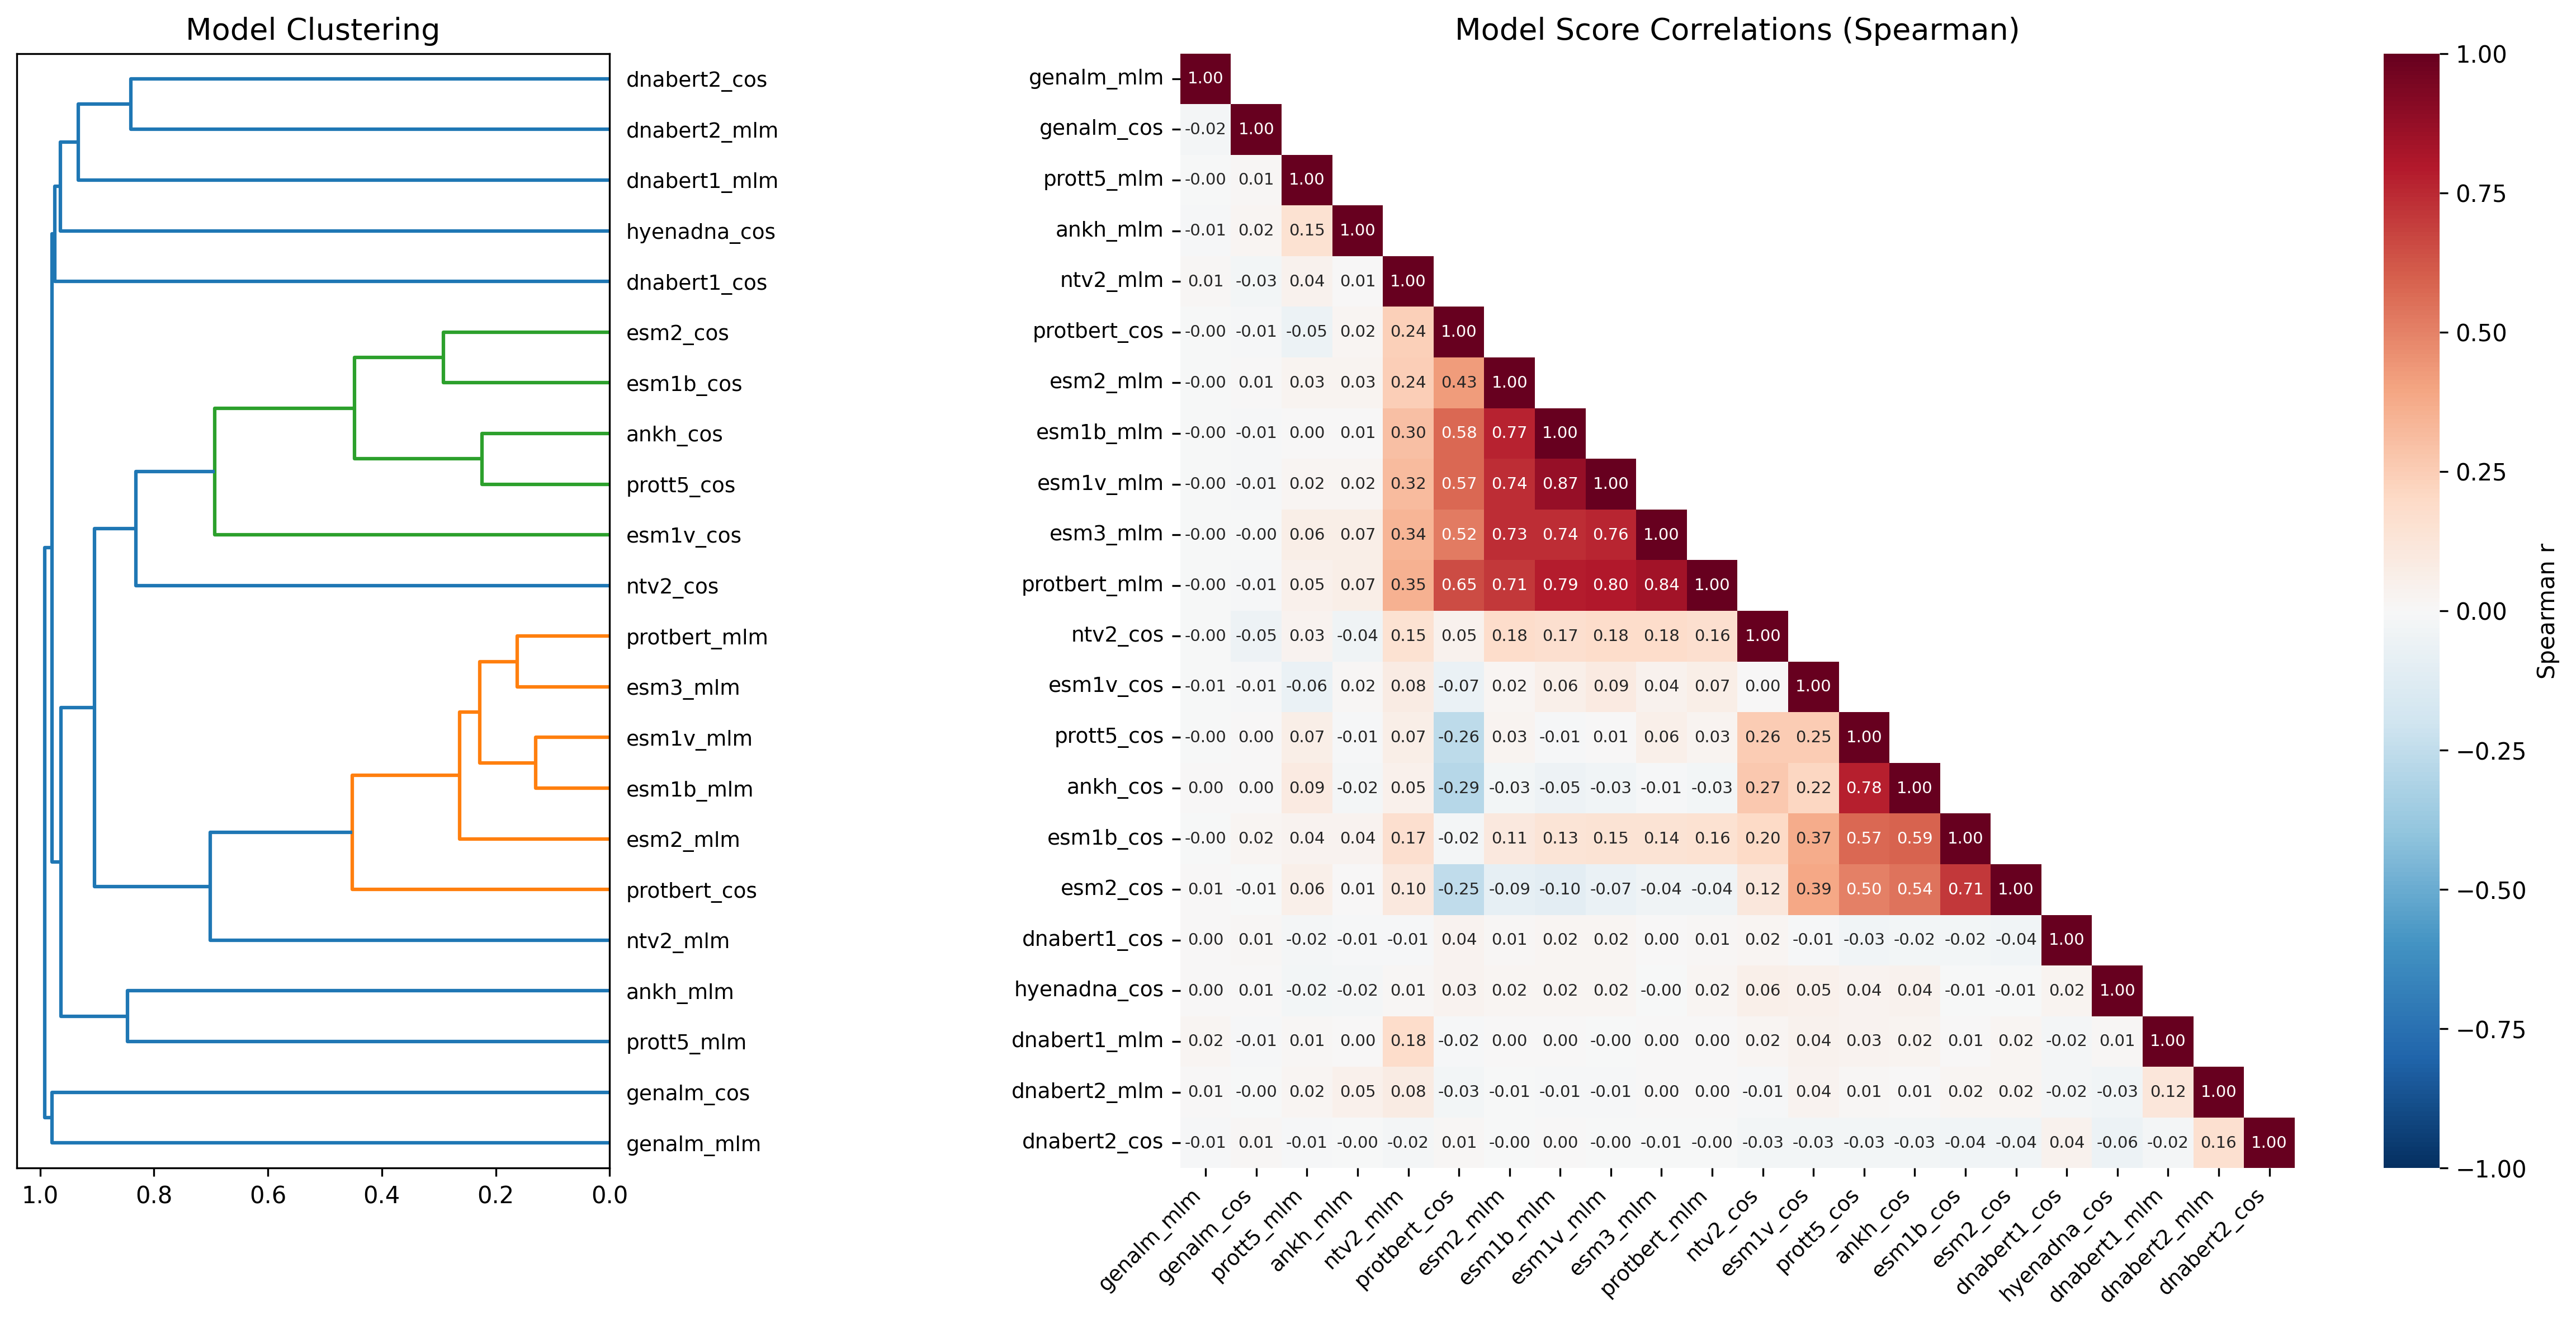
\includegraphics[width=0.7\textwidth]{figures/fig1_correlation_heatmap.png}
    \caption{Pairwise Spearman correlation. Protein MLM models are highly correlated ($r = 0.68$--$0.83$). Nucleotide models are nearly orthogonal to protein models ($r \approx 0.00$).}
    \label{fig:correlation}
\end{figure}

Key findings: intra-protein MLM $r = 0.393 \pm 0.366$, intra-nucleotide MLM $r = 0.071 \pm 0.065$, cross-modality $r = 0.059 \pm 0.120$.

\subsection{Variant Difficulty and Biological Correlates}

\begin{figure}[h]
    \centering
    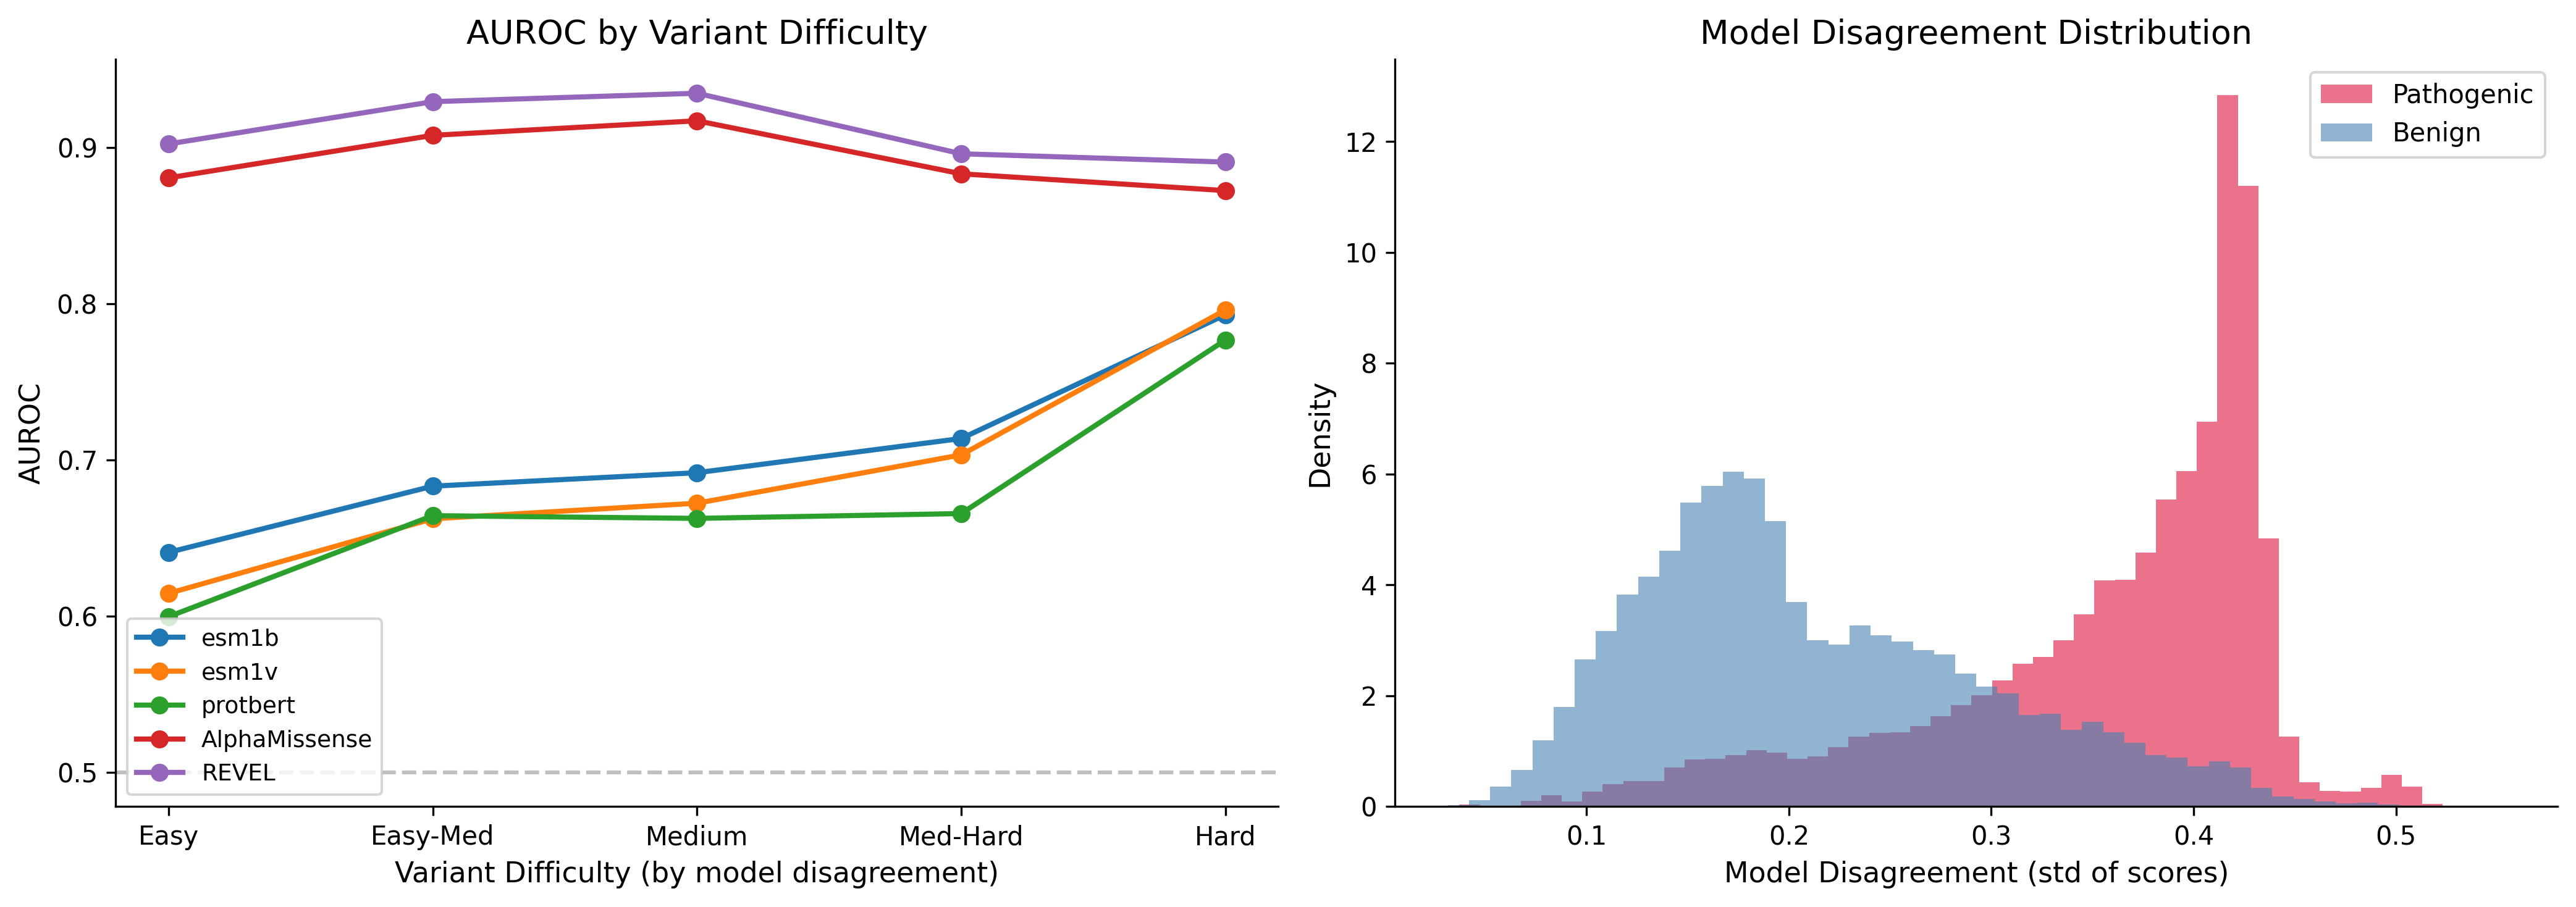
\includegraphics[width=0.7\textwidth]{figures/fig2_difficulty_spectrum.png}
    \caption{Performance across the variant difficulty spectrum. Models degrade on variants with high cross-modal disagreement.}
    \label{fig:difficulty}
\end{figure}

\begin{figure}[h]
    \centering
    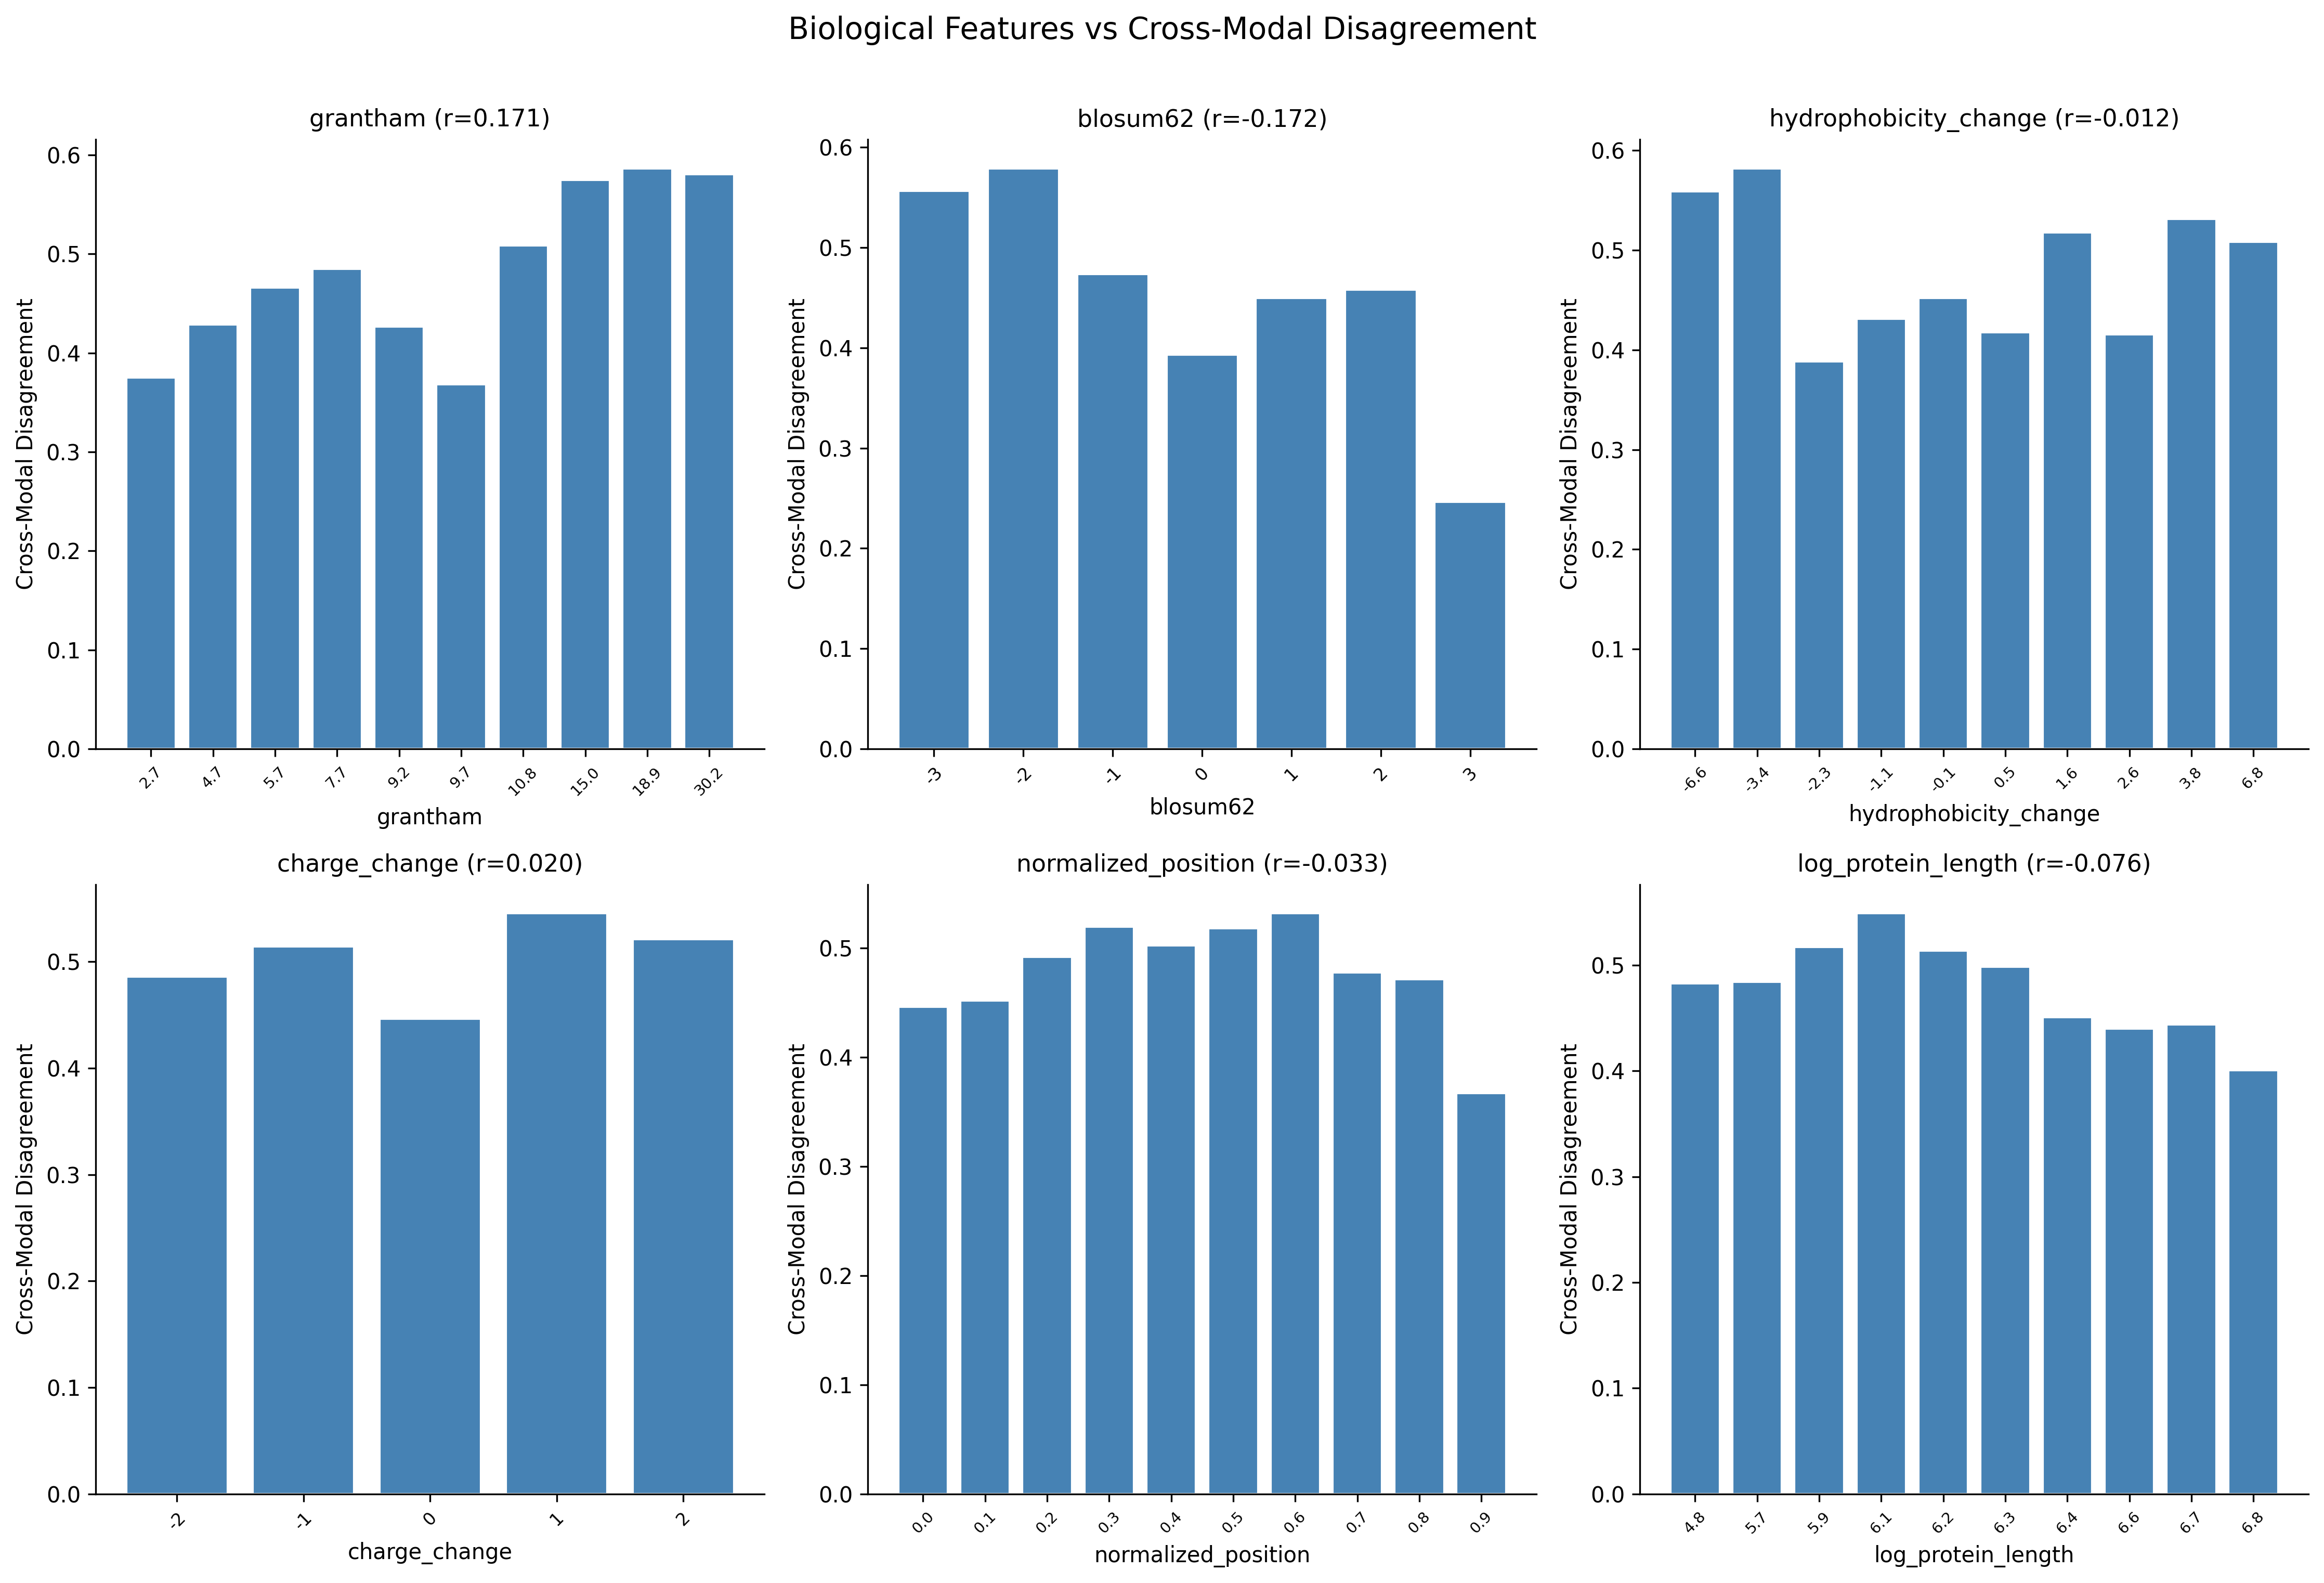
\includegraphics[width=0.7\textwidth]{figures/fig3_biological_correlates.png}
    \caption{Biological correlates of cross-modal disagreement.}
    \label{fig:biology}
\end{figure}

BLOSUM62 ($r = -0.181$), Grantham distance ($r = 0.180$), cysteine changes ($r = 0.142$), and protein length ($r = -0.110$) are the strongest correlates of variant difficulty.

\subsection{Fusion Ablation}

\begin{table}[h]
\centering
\caption{Fusion ablation under gene-disjoint evaluation.}
\label{tab:ablation}
\small
\begin{tabular}{lrrr}
\toprule
\textbf{Configuration} & \textbf{N feat.} & \textbf{AUROC} & \textbf{MCC} \\
\midrule
Best Single (ESM1b-MLM) & 1 & 0.881 & 0.608 \\
Protein MLM Only & 5 & 0.910 & 0.665 \\
All Protein (MLM+Cos) & 11 & 0.924 & 0.698 \\
Nucleotide MLM Only & 4 & 0.650 & 0.201 \\
All Nucleotide (MLM+Cos) & 9 & 0.699 & 0.280 \\
\midrule
All Foundation Models & 20 & 0.928 & 0.707 \\
Foundation + Physicochemical & 23 & 0.931 & 0.715 \\
\midrule
Meta-Learner (Ours) & 29 & \textbf{0.933} & \textbf{0.723} \\
\bottomrule
\end{tabular}
\end{table}

The meta-learner (0.933) approaches AlphaMissense (0.948) without population frequency data. Adding nucleotide models yields marginal gains (+0.004), confirming orthogonality.

\subsection{Representation Geometry: CKA}

We analyze internal representations using Centered Kernel Alignment (CKA) \cite{kornblith2019similarity} with an RBF kernel (median heuristic for bandwidth).

\begin{figure}[h]
    \centering
    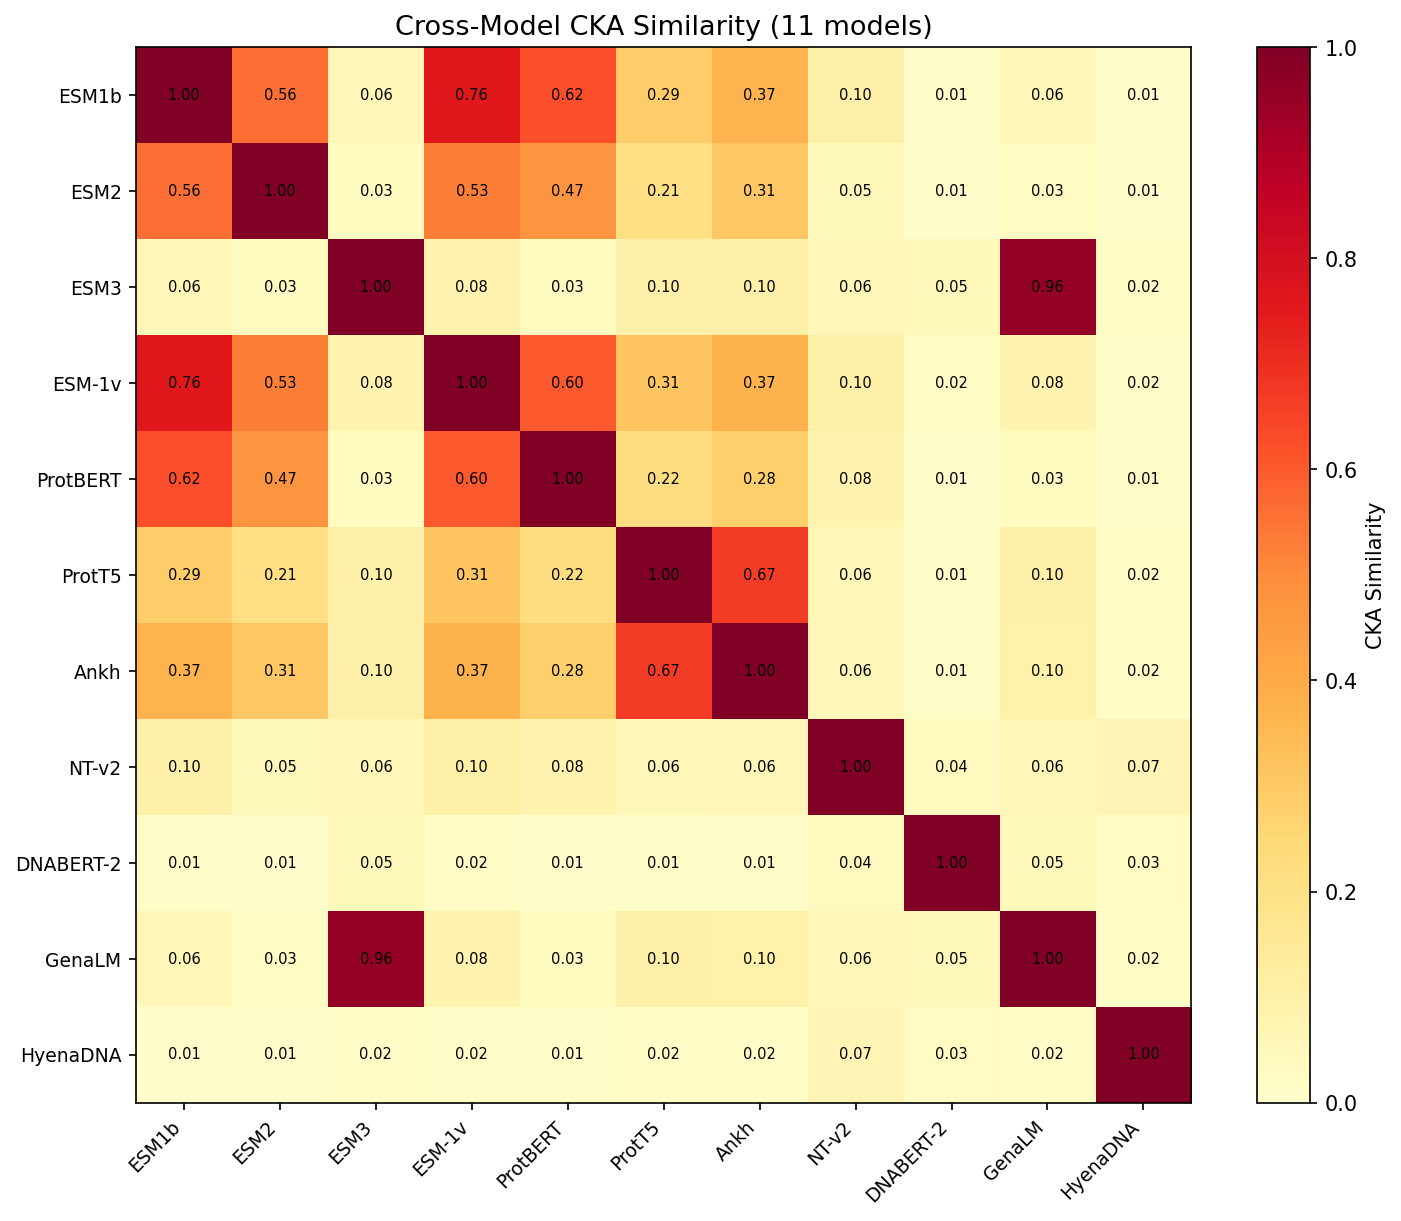
\includegraphics[width=0.7\textwidth]{figures/fig_cka_cross_model.png}
    \caption{Cross-model CKA (median-heuristic RBF). Protein models cluster (upper-left); cross-modality CKA $<$ 0.104.}
    \label{fig:cka_cross}
\end{figure}

Key CKA values: ESM1b--ESM-1v = 0.772, ESM1b--ProtBERT = 0.638, ProtT5--Ankh = 0.671. Cross-modality mean = 0.044 (range 0.005--0.104). Nucleotide intra-cluster mean = 0.047.

\begin{figure}[h]
    \centering
    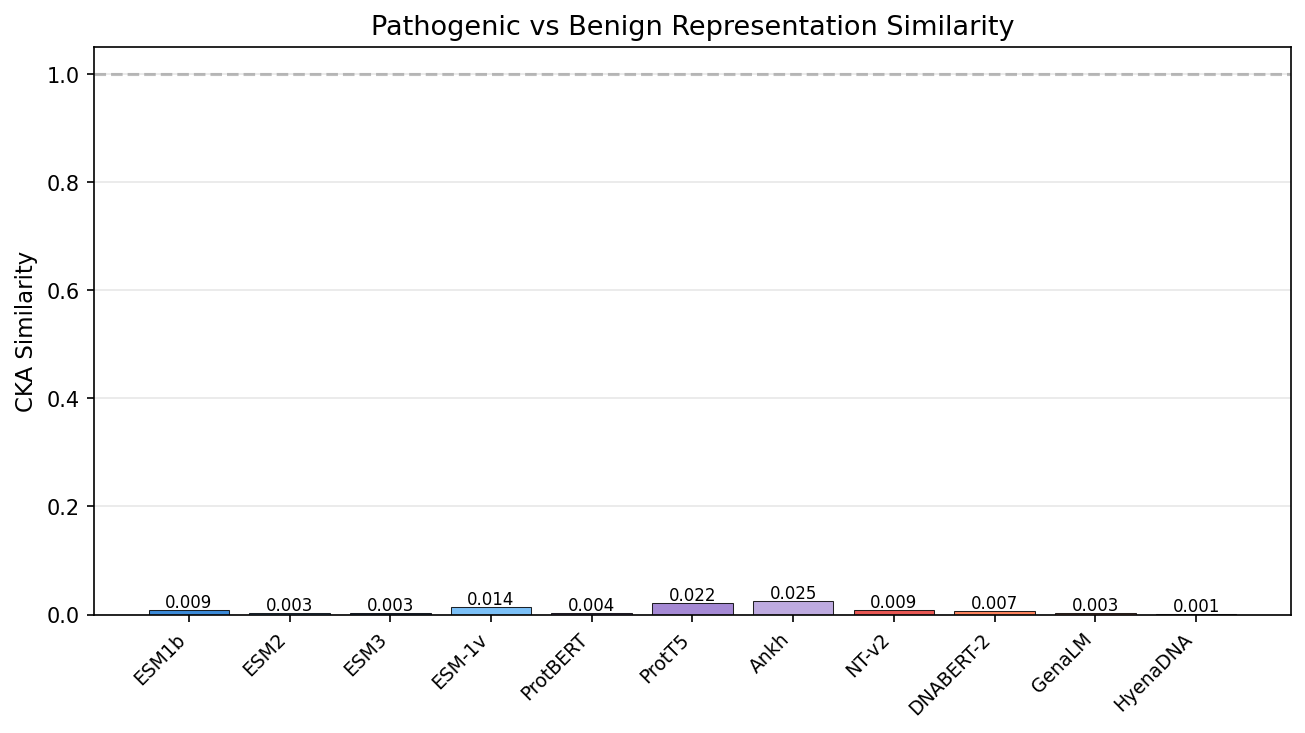
\includegraphics[width=0.7\textwidth]{figures/fig_pathogenic_benign_cka.png}
    \caption{CKA between pathogenic and benign representations. All models show CKA $<$ 0.025, indicating pathogenicity is encoded through geometric reorganization.}
    \label{fig:cka_pathben}
\end{figure}

All models show CKA $<$ 0.025 between pathogenic and benign variants, indicating discriminative representations via geometric reorganization rather than magnitude changes.

\begin{figure}[h]
    \centering
    \begin{subfigure}[b]{0.48\textwidth}
        \centering
        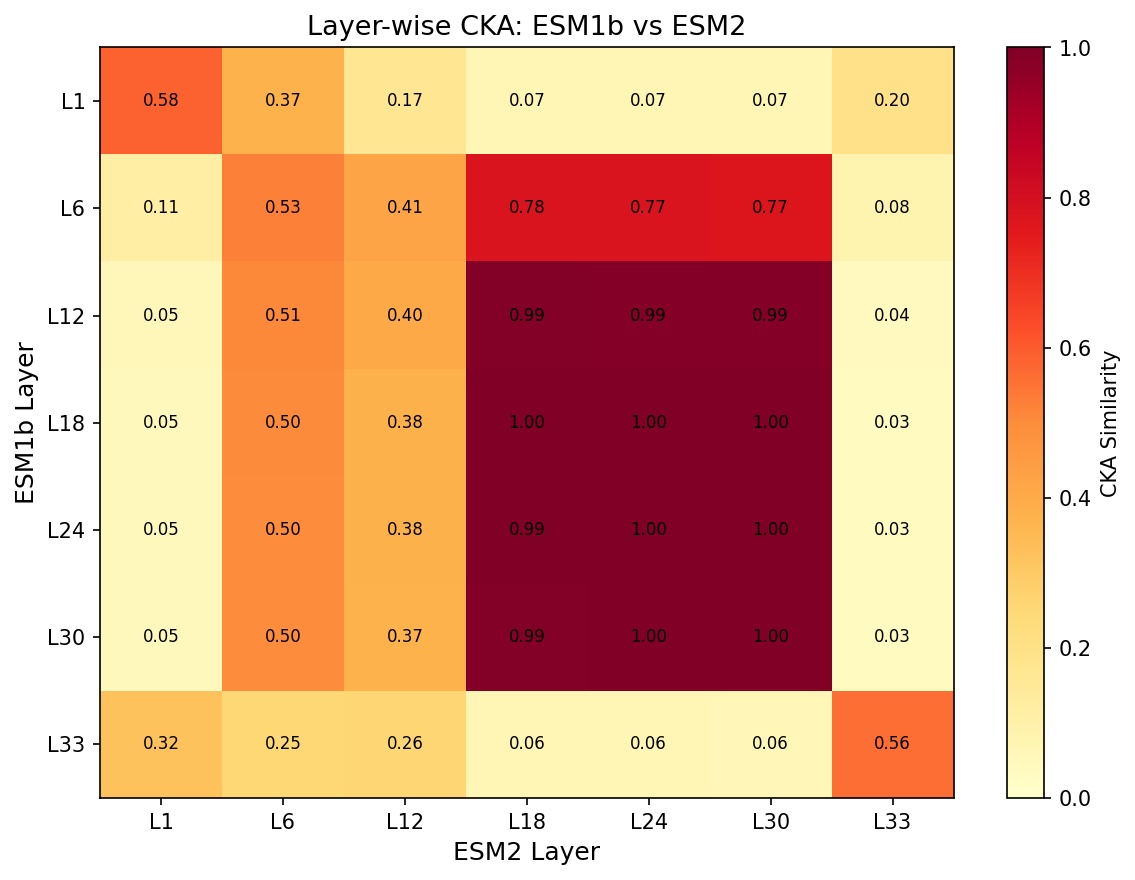
\includegraphics[width=\textwidth]{figures/fig_cka_layerwise_heatmap.png}
        \caption{Layer-wise CKA (ESM1b vs ESM2)}
        \label{fig:cka_layerwise}
    \end{subfigure}
    \hfill
    \begin{subfigure}[b]{0.48\textwidth}
        \centering
        
\includegraphics[width=\textwidth]{figures/fig_layerwise_probing.png}
        \caption{Layer-wise pathogenicity probing}
        \label{fig:layerwise_probing}
    \end{subfigure}
    \caption{Left: Layer-wise CKA between ESM1b and ESM2 (final-layer CKA = 0.598). Right: Pathogenicity probing accuracy increases monotonically from L1 ($\approx$0.72) to L33 ($\approx$0.81).}
    \label{fig:layerwise}
\end{figure}

\subsection{Linear Probing}

\begin{figure}[h]
    \centering
    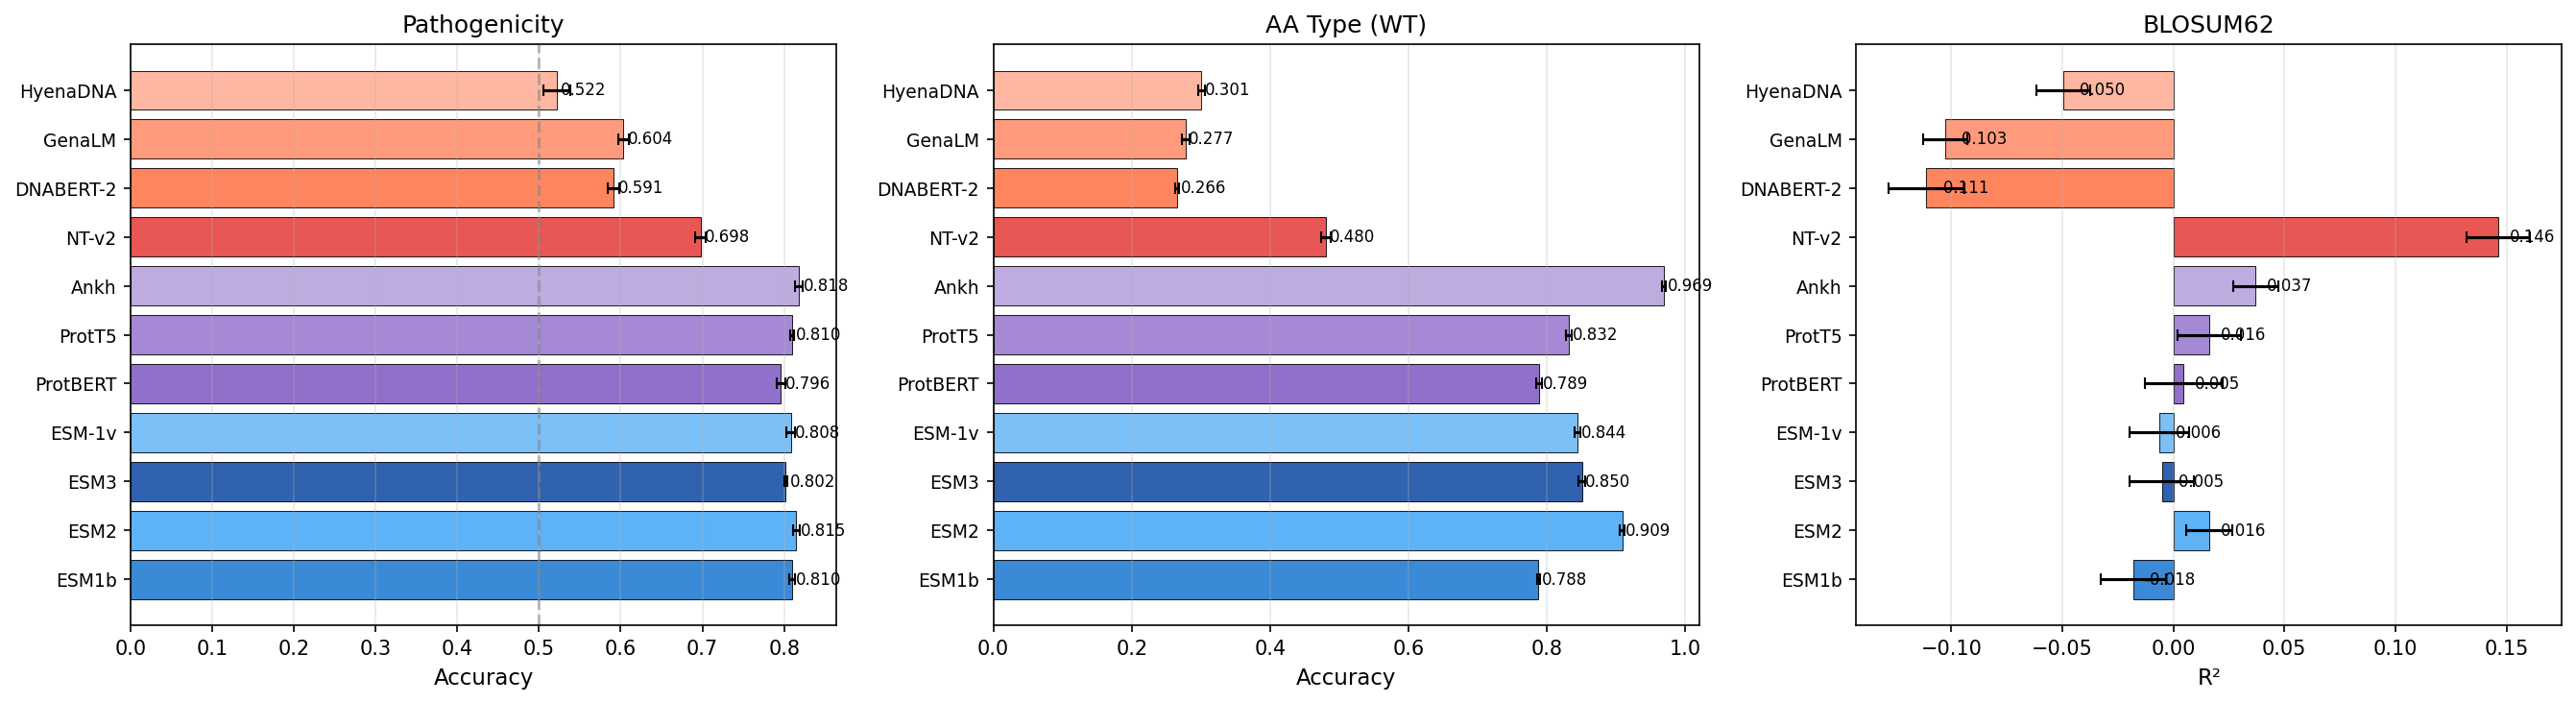
\includegraphics[width=0.7\textwidth]{figures/fig_probing_tasks.png}
    \caption{Linear probing on three tasks. Protein models outperform nucleotide models on pathogenicity. Ankh achieves 0.968 accuracy on AA type.}
    \label{fig:probing}
\end{figure}

Protein models achieve 0.80--0.82 pathogenicity AUROC; nucleotide models range from 0.52--0.70. On AA type, Ankh reaches 0.968, while nucleotide models score 0.27--0.48 (vs. chance 0.05), confirming they do not encode amino acid identity.

\section{Discussion}

\paragraph{Protein models dominate.} ESM1b-MLM (AUROC 0.882) far exceeds the best nucleotide model (NT-v2 at 0.639). Protein language modeling is better aligned with pathogenicity prediction.

\paragraph{Orthogonality enables fusion.} Low cross-modality correlation ($r \approx 0.00$) and CKA (mean 0.044) indicate complementary variant information. However, the marginal fusion gain (+0.004) suggests nucleotide signal is limited for missense variants.

\paragraph{Pathogenicity as geometric reorganization.} All models show CKA $<$ 0.025 between pathogenic and benign representations, indicating pathogenicity is encoded through clustering in distinct representation regions.

\paragraph{Layer-wise accumulation.} Pathogenicity probing improves monotonically from L1 ($\approx$0.72) to L33 ($\approx$0.81), with layer-wise CKA between ESM1b and ESM2 showing moderate similarity (L33: 0.598).

\paragraph{Limitations.} (1) D2 genes are a subset of D1 genes; temporal validation tests the same genes at a different time point rather than truly unseen genes. (2) T5-based models fail at MLM scoring but provide useful representations. (3) We evaluate only on missense variants. (4) The gene-disjoint protocol may underestimate clinical performance where gene-level information is available.

\section{Conclusion}

We provide the first controlled multi-modal benchmark comparing protein and nucleotide foundation models under gene-disjoint evaluation, with representation analysis via CKA and linear probing. Protein MLM models capture a shared high-performance signal; nucleotide models are orthogonal (mean CKA = 0.044) but provide limited additional signal for missense variants. All models encode pathogenicity through geometric reorganization. A lightweight meta-learner (AUROC 0.933) approaches AlphaMissense without population frequency data.

\bibliographystyle{plainnat}
\bibliography{references}

\end{document}
